\chapter{Final conclusions and further work}\label{cap:conclusiones}

\subsection{What's coming next for farmOS: version 2.0}
Walking through these pages, we have been able to learn about the enormous potencial that farmOS has. Not only because of the way the software ifself has been developed but also because it is a Drupal distribution, which means is free software. Free as in freedom, of course.

As it has been mentioned before, he fact that it is licensed with GPLv2 allows us to enjoy the four freedom all free software offers to both the user and the developer: we are able to use, study, copy and improve the software in whatever way it is considered appropiate.

However, what is the next step for farmOS? It is worth mentioning the direction the project is currently taking as version 2.0 is closer to be released.

\vspace{3mm}

\begin{figure}[H]
    \centering
    
\includegraphics[width=0.3\textwidth]{fig/new-farmos.png}
    \caption{New farmOS logo for version 2}
    \label{fig:new-farmos}
\end{figure}

\vspace{3mm}

\subsubsection{Why farmOS 2.x?}
One of the fundamental reasons why farmos is upgrading to a version 2 is because of the end of Drupal 7.

Let me quote what the maintainers have commented on this topic\cite{end-of-d7}.

\vspace{3mm}
-----------------------------------------------------------------------

`` farmOS is currently built on Drupal 7, which was released in 2011 and will be end-of-life in November 2021 2022. This means it will no longer be supported by the Drupal community.

In the meantime, Drupal 8 (released in 2015) and Drupal 9 (released in 2020) offer significant improvements that farmOS will benefit greatly from.''

-----------------------------------------------------------------------
\vspace{3mm}

The main motivation\cite{farmosv2} of this new version is to offer a new user interface that will improve the user experience as well. Furthermore, there are another features that are being included such as translation and localization capabilities.

One of the major differences with regard to the previous version is that areas are now going to belong to assets, more concretely location type assets.

There are also going to be some changes for developers using and contributing to farmOS. There will be improvements to backend APIs, documentation, modules and other integrations.

We have also installed a brand-new farmOS v2 and, although we will not get any deeper, we wanted to take a look at the general view of how the main screen is looking.

\vspace{3mm}

\begin{figure}[H]
    \centering
    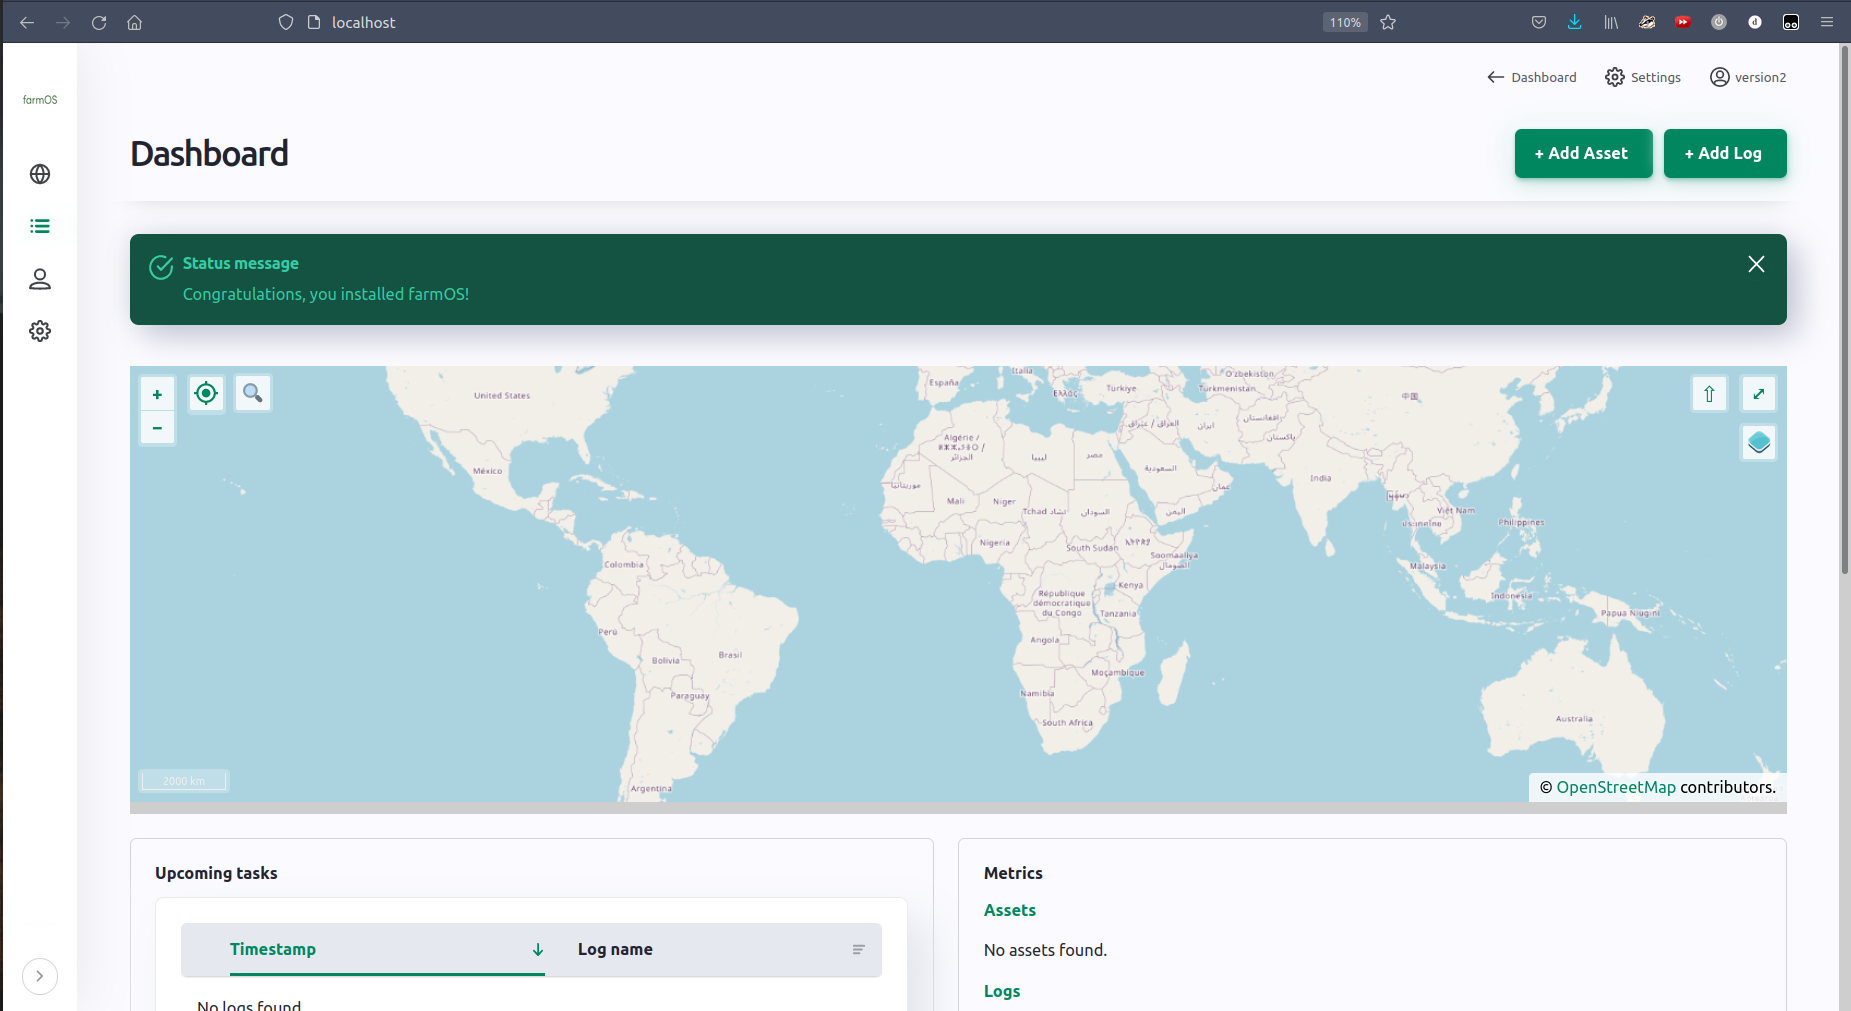
\includegraphics[width=1.07\textwidth]{fig/brandnew-farmosv2.png}
    \caption{General view of main page in farmOS v2}
    \label{fig:brandnew-farmosv2}
\end{figure}

\vspace{3mm}

For what is worth, the installation has also become significantly simpler. Here are the \href{https://docs.farmos.org/development/environment/}{steps}

In the case that the reader is eager to obtain some more information in relation to this new release that is being cooked, here's the new \href{https://docs.farmos.org/model/}{documentation link}.

